%UNIT 3: AN ANALYTIC APPROACH
%%%%%%%%%%%%%%%%%%%%%%%%%%%
%%%% Put the following at the top of each .tex file  %
\pagestyle{fancy}
\renewcommand{\theUnit}{4.2}
\ifthenelse{\isundefined{\UnitPageNumbers}}{}{\setcounter{page}{1}}
\rhead{Application  \theUnit: Heating and Cooling}
\lhead{
\includegraphics[width=1.25cm]{IODE-logo.png}}
\rfoot{\mypage}
\lfoot{}
\cfoot{}
\fancypagestyle{firstfooter}{\footskip = 50pt}
\renewcommand{\footrulewidth}{.4pt}
%%%%%%%%%%%%%%%%%%%%%%%%%%%
\vspace*{-20pt} \thispagestyle{firstfooter}
\pagebegin{Cooling Coffee}

%
\includegraphics[]{../../IODE/Tex/Originals/07/07CoffeeCup.png}
A group of students want to develop a rate of change equation to describe the cooling rate for hot coffee in order that they can make predictions about other cups of cooling coffee. Their idea is to use a temperature probe to collect data on the temperature of the coffee as it changes over time and then to use this data to develop a rate of change equation. \\

The data they collected is shown in the table below. The temperature $C$ (in degrees Fahrenheit) was recorded every 2 minutes over a 14 minute period. \\

\begin{tabular}{|c|c|c|}
\hline
Time (min) & Temp. (\degree F) & $\frac{dC}{dt}$ (\degree F per min) \\\hline
0 & 160.3 & \ \ \ \ \ \ \ \ \ \ \ \ \ \ \ \ \ \ \ \  \\\hline
2 & 120.4 & \\\hline
4 & 98.1 &\\\hline
6 & 84.8 & \\\hline
8 & 78.5 & \\\hline
10 & 74.4 & \\\hline
12 & 72.1 & \\\hline
14 & 71.5& \\\hline
\end{tabular}
  
  \bb
  \ii Figure out a way to use this data to fill in the third column whose values approximate  $\displaystyle\frac{dC}{dt}$, where $C$ is the temperature of the coffee.\label{07problem1} 
  \item Do you expect $\displaystyle\frac{dC}{dt}$ to depend on just the temperature $C$, on just the time $t$, or both the temperature $C$ and the time $t$? \label{07problem2} 

\item Sketch below your best guess for the graph of $\displaystyle\frac{dC}{dt}$. \label{07problem3}
\begin{center}
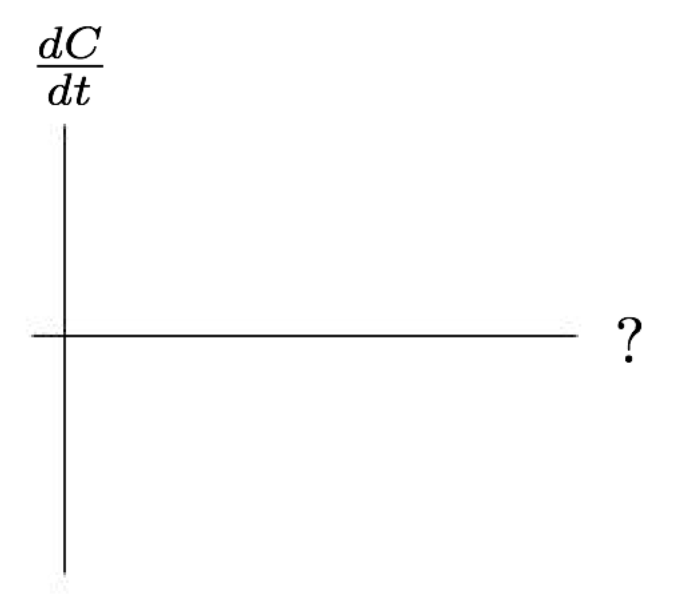
\includegraphics[width=2.5in]{Originals/07/07dCdt.png}
\end{center}
    
\clearpage
\pagebegin{Newton's Law of Heating and Cooling}

\item \
\begin{enumerate} \label{07problem4} 
\item Input the data from your extended table in question \ref{07problem1} into the GeoGebra applet \\\href{https://ggbm.at/uj2gbz3V}{\underline{https://ggbm.at/uj2gbz3V}} to plot points for $\displaystyle\frac{dC}{dt}$ vs. $C$. Does this plot confirm or reject your sketch from question \ref{07problem3}? 
\vspace{1.5in}
\item Toggle on the curve fitting tool and find an equation that fits your data.
\end{enumerate} 
\ee

\vspace{-2in}\hspace{-0.5in}
\includegraphics[width=0.5in]{Originals/07/07CoolingCoffeeQR.png}
\vfill


\bbox
\alert{Newton's Law of Heating and Cooling} states that the temperature $T$ of an object at time $t$
changes at a rate which is proportional the difference of its temperature and the
temperature of its surrounding:
\[ \frac{dT}{dt} = -k(T-A) \]
 where $A$ is a constant that denotes the ambient temperature and $k>0$ is a constant that depends on the object.
\ebox

\bb[resume]
\ii What happens as $\mathbf{t \to \infty}$ if the initial temperature $\mathbf{T_0>A}$? If $\mathbf{T_0 < A}$? \vfill


%\ii What is/are the equilibrium solution(s)?
%\ii Find a general solution to the differential equation. Your formula for $T$ will depend on the constants $k$ and $A$ as
%well as the an arbitrary constant $C$.
%\ee

\clearpage

\pagebegin{Practice: Applications to Economics}

\ii %http://www.math.lamar.edu/faculty/maesumi/applied\%20calculus/hoffman/ch05sec03.pdf
Let $S(p)$ denote the number of units of a particular commodity supplied to the market at a price of $p$ dollars per unit, and let $D(p)$ denote the corresponding number of units demanded by the market at the same price.
\bi
\ii In static circumstances, market equilibrium occurs at the price where demand equals supply.
\ii However, certain economic models consider a more dynamic economy in which price, supply, and demand are assumed to vary with time.
\ii One of these, the Evans price adjustment model, assumes that the rate of change of price with respect to time $t$ is proportional to the shortage, which is the difference between the quantity demanded and the quantity supplied..
\ei

\bb
\ii Write a differential equation for the rate of the change of the price of the good with respect to time. \vspace{1in}
\ii If we assume that supply and demand are linear functions given by 
\[ S(p) = 2+p \ \ \ \ \mbox{ and } \ \ \ D(p)=8-2p, \]
Find a general solution to the differential equation in part (a). \vfill
\ii If the price is \$$5$ at time $t=0$ and \$$3$ at time $t=2$, determine what happens to $p$ in the long run. \vfill
\ee

\clearpage

\pagebegin{Practice: Applications to Forensic Science}

\ii %11-5y39
A detective finds a murder victim at 9 am. The temperature of the body
is measured at $90.3^{\circ}$F. One hour later, the
temperature of the body is $89.0^{\circ}$F. The
temperature of the room has been maintained at a constant
$68^{\circ}$F.
\bb
\ii Assuming the temperature, $T$, of the body obeys Newton's Law of
Cooling, write a differential equation for $T$. Your equation will include
the constant $k$ (for now). \vspace{1.25in}
\ii Solve the differential equation to estimate the time the murder occurred. \vfill
\ee
\ee
